\documentclass{article}

\usepackage[T1]{fontenc}
\usepackage{amsmath}
\usepackage{amssymb}
\usepackage{graphicx}
\usepackage{titling}
\usepackage{ragged2e}
\usepackage{lipsum}
\usepackage{booktabs}
\usepackage{verbatim}
\usepackage[hidelinks]{hyperref}
\usepackage[a4paper,left=0.75in,right=0.75in,top=1in,bottom=1in,footskip=0.5in]{geometry}

\pretitle{\vspace{1in}\hrulefill\par}
\posttitle{\par\hrulefill}

\title{\begin{center}\Huge COMP2432\\
    G06 Group Project Reoprt\end{center}}
\date{}
\author{}

\begin{document}
    \begin{titlepage}
        \maketitle
        \begin{center}
            \huge Room Booking Manager
            \vfill
            \begin{table}[!htbp]
                \centering
                \huge
                \begin{tabular}{ll}
                    19081789D\hspace{0.25in}&MAN, Furui \\
                    19078543D\hspace{0.25in}&WANG, Meng \\
                    18080998D\hspace{0.25in}&WU, Junyu  \\
                    19079008D\hspace{0.25in}&XING, Shiji\\
                \end{tabular}
            \end{table}
            \vspace{0.5in}
            \thispagestyle{empty}
        \end{center}
    \end{titlepage}
    \cleardoublepage
    \tableofcontents
    \thispagestyle{empty}
    \cleardoublepage
    \setcounter{page}{1}
    \section{Introdoction}
        \paragraph{}
        The project aims to utilize the knowledge covered in COMP2432 Operating Systems
        and put them into practice to get a further understanding and improvement. This
        works out by implementing a facility management system for a company, which
        would make advantage of all kinds of scheduling skills and abstractions covered
        in the lecture, along with the use of multi-process programming and inter-process
        communication. 
    \cleardoublepage
    \section{Scope}
        \paragraph{}
        Multi-Process Programming and Inter-process Communication: pipe() and fork(); 
        \paragraph{}
        CPU Scheduling: FCFS and PR 
        \paragraph{}
        Memory Allocation: MFT
        \paragraph{}
        Synchronization: Program-Monitored Synchronization 
    \cleardoublepage
    \section{Concept}
        \subsection{FCFS Scheduling}
            \paragraph{}
                FCFS scheduling is indeed taking the arriving time of the request as the
                priority. It is very easy to implement this algorithm, as long as the
                order of the request array is the same order as input, which is very
                natural. One thing to note that to keep the order of request array the
                same as input order, Input Module must be single-threaded. 
        \subsection{PRIO Scheduling}
            \paragraph{}
            It is already mentioned that FCFS is a special case of PRIO scheduling where
            the priority is the arriving time. Now that a priority is appended with the
            request, all it needs is to sort the request array by priority, then call
            FCFS scheduling to implement PRIO scheduling. This reuses the code and
            decrease the complexity of the program. 
    \cleardoublepage
    \section{Design of opti}

    \cleardoublepage
    \section{Program Structure}
        \subsection{Class Design}
            \begin{figure}[!htbp]
                \centering
                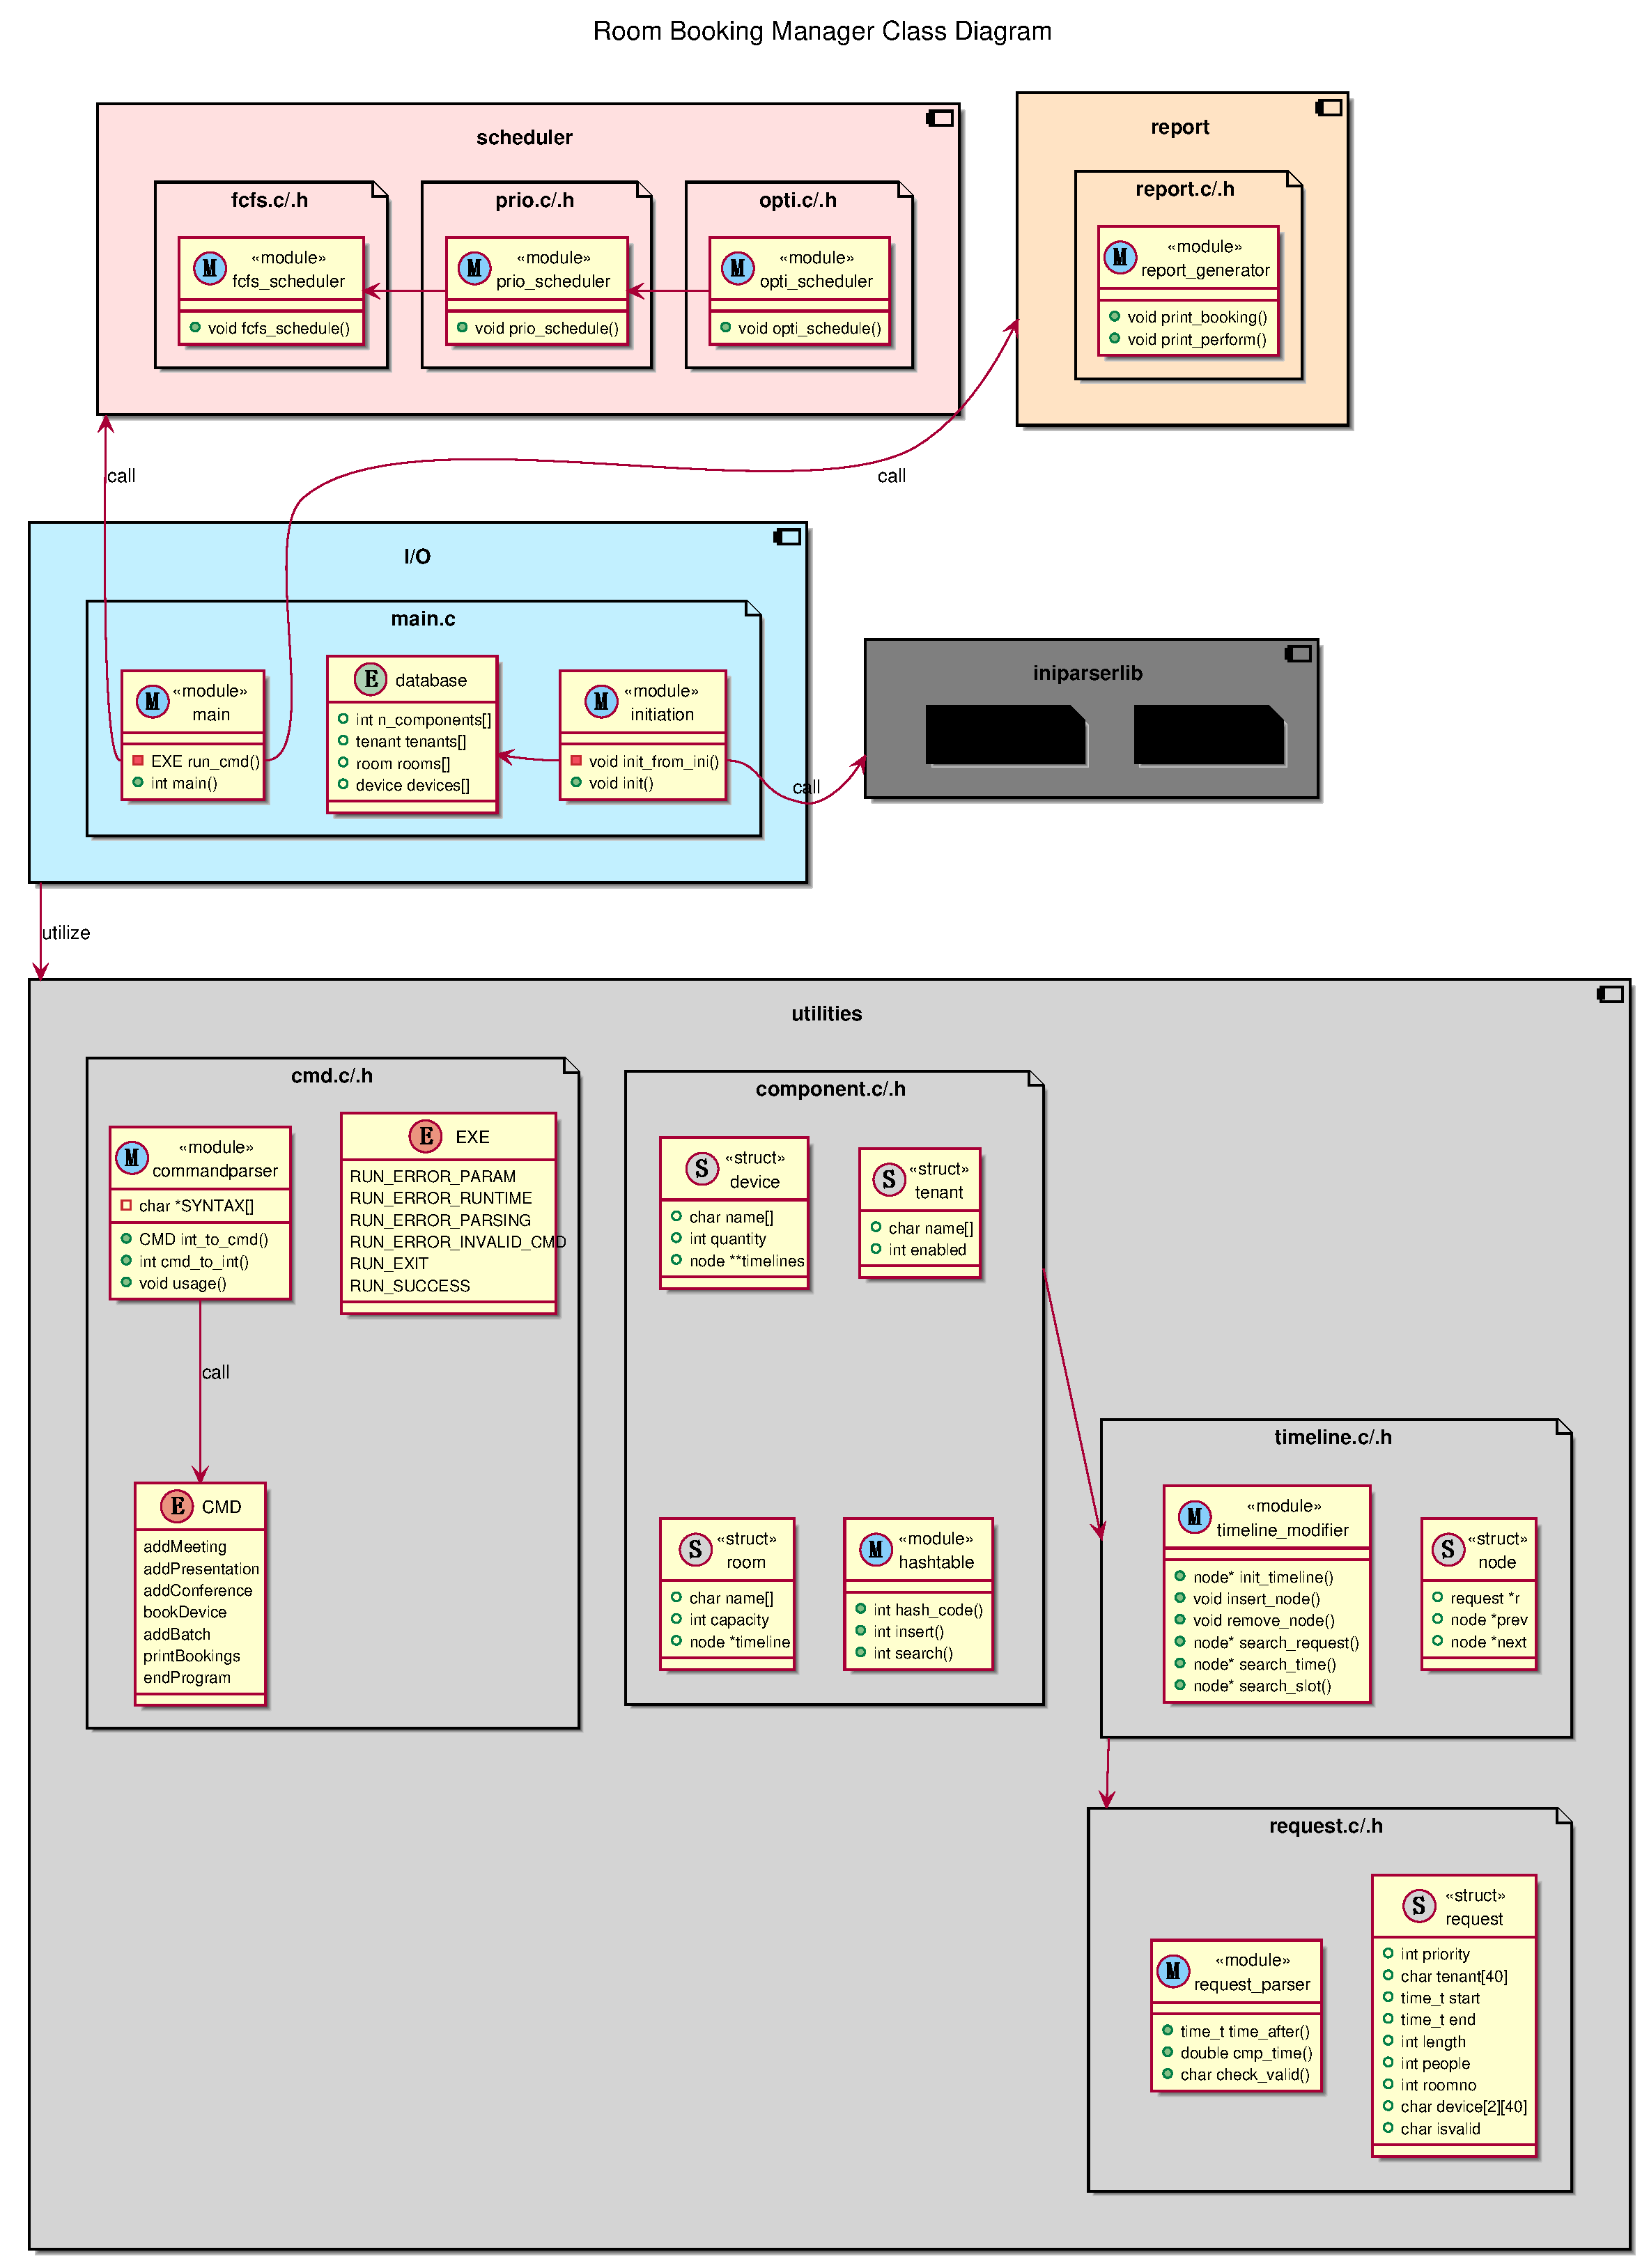
\includegraphics[scale=0.4]{./img/eps/class_diagram.eps}
                \caption{Overall class design diagram of Room Booking Manager}
            \end{figure}
        \subsection{Sequence Design}
            \begin{figure}[!htbp]
                \centering
                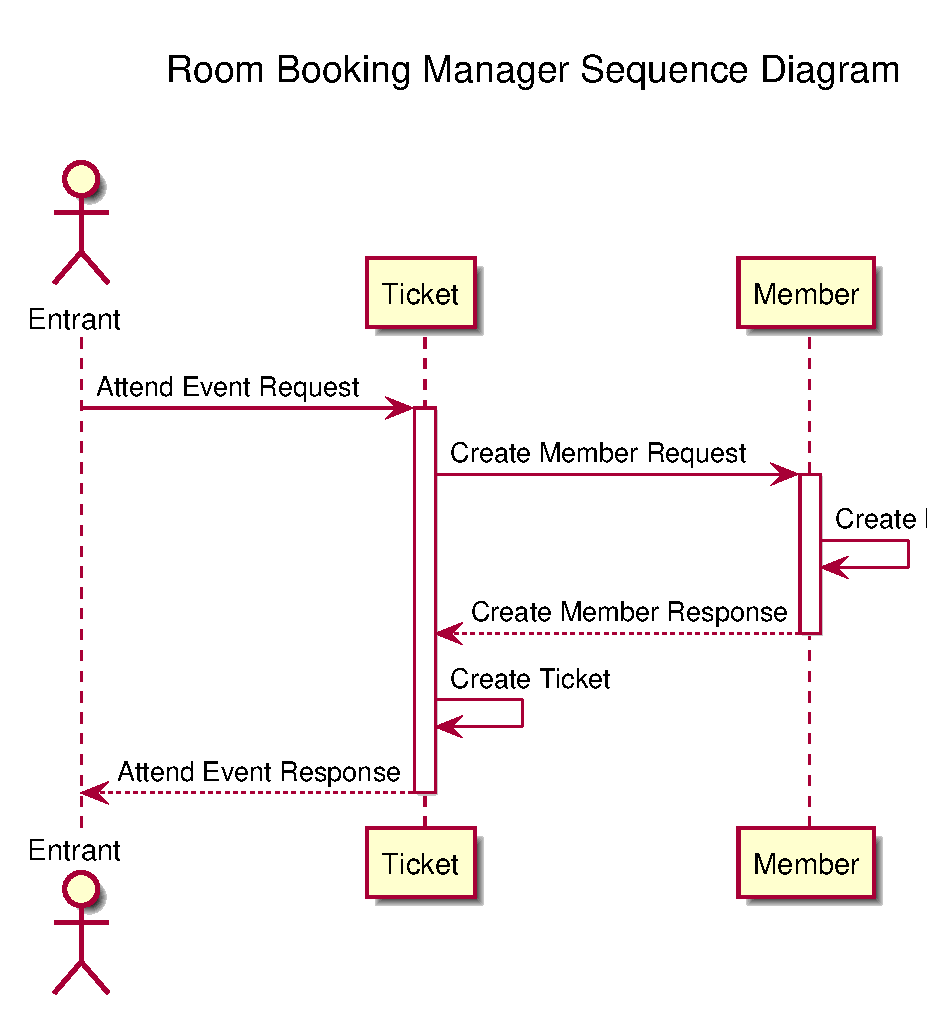
\includegraphics[scale=0.5]{img/eps/sequence_diagram.eps}
                \caption{Overall sequence design diagram of Room Booking Manager}
            \end{figure}
        \subsection{Activity Design}
            \begin{figure}[!htbp]
                \centering
                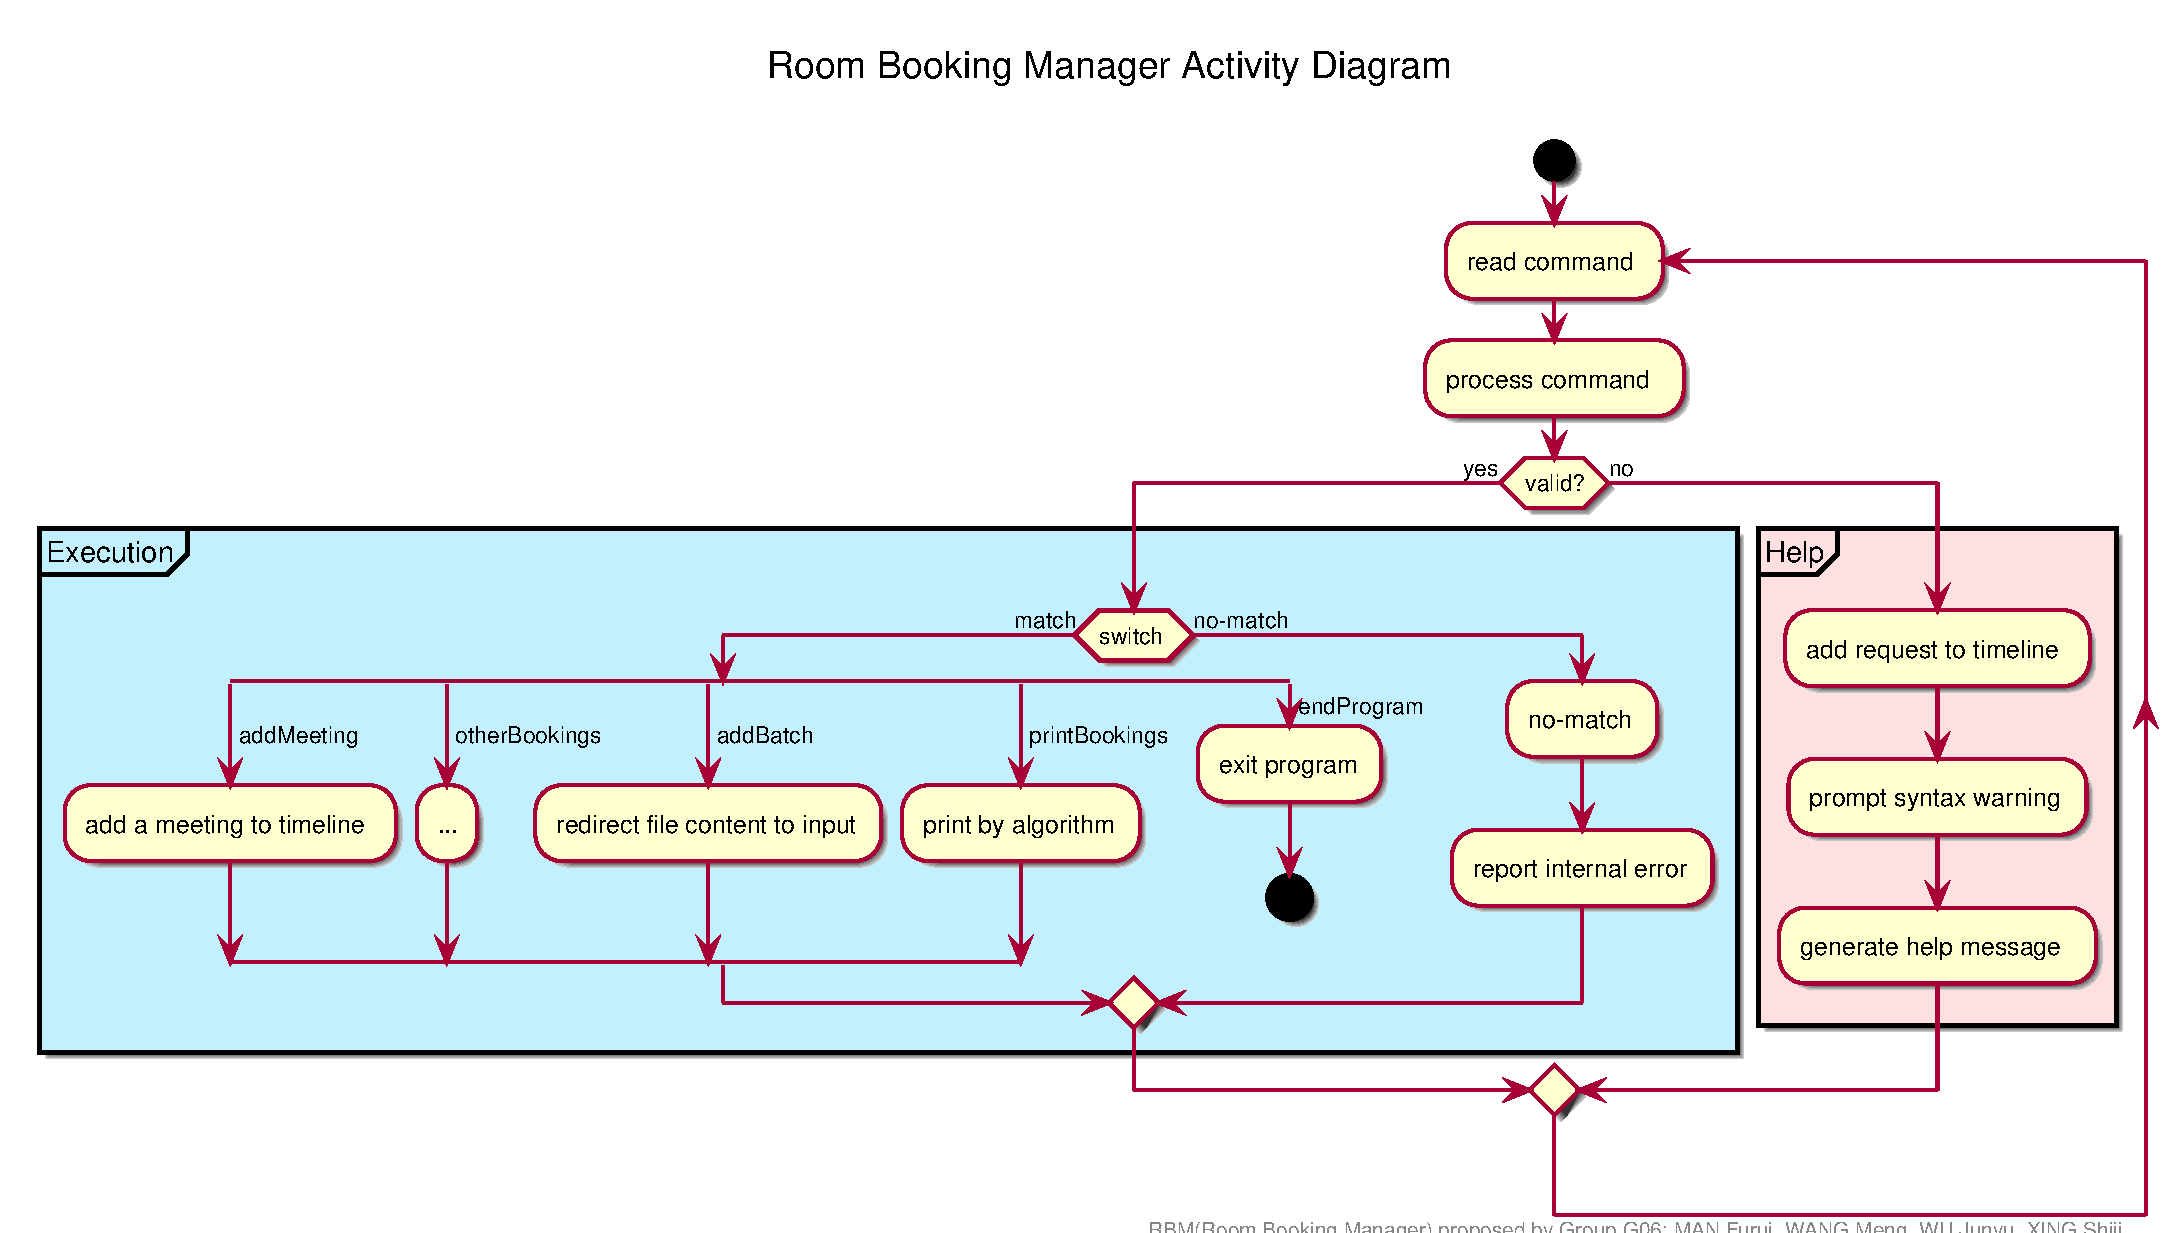
\includegraphics[scale=0.45]{img/eps/activity_diagram.eps}
            \end{figure}

    \cleardoublepage
    \section{Testing Cases}
        \paragraph{}
        This is the brief version. 
        \paragraph{}
        Below demonstrates the valid and invalid tests for addMeeting instruction.
        \paragraph{}
        Tests for other instructions are similar but vary in parameters. 
        \paragraph{}
        Refer to appendix for full version. 

        \paragraph{valid tests}
        \begin{verbatim}
            // the valid syntax is: 
            // addMeeting –tenant YYYY-MM-DD hh:mm n.n [d1 d2]; 
            addMeeting -tenant_A 2021-05-10 21:50 1.50 5 projector_2K screen_100;
            addMeeting -tenant_A 2021-05-11 18:20 0.30 5;
            addMeeting -tenant_A 2021-05-11 4:10 0.0 5;
        \end{verbatim}
        
        
        \paragraph{invalid tests}
        \begin{verbatim}
            // invalid instructions are either:
            // command is invalid
            command_invalid and parameters does not matter;
            // tenant invalid
            addMeeting -tenant_invalid 2021-05-10 1:30 0.50 5 projector_2K screen_100;
            // date invalid
            addMeeting -tenant_A date-in-valid 1:30 0.50 5 projector_2K screen_100;
            // hhmm invalid
            addMeeting -tenant_B 2021-05-10 hhmm:invalid 1.50 5 webcam_FHD monitor_75;
            // duration invalid 
            addMeeting -tenant_C 2021-05-10 18:30 duration.invalid 5 webcam_FHD monitor_50;
            // people invalid
            addMeeting -tenant_D 2021-05-10 10:40 0.0 peopleinvalid projector_2K screen_150;
            // device invalid
            addMeeting -tenant_D 2021-05-16 3:10 1.10 5 device_invalid monitor_50;
            // device pairing invalid 
            addMeeting -tenant_E 2021-05-10 22:20 0.50 5 projector_4K monitor_50; 
            // device without pairing 
            addMeeting -tenant_E 2021-05-10 22:20 0.50 5 projector_4K; 
        \end{verbatim}

    \cleardoublepage
    \section{Performance analysis}

    \cleardoublepage
    \section{Program Setup \& Analysis}
        \subsection{Program Setup}
            \paragraph{Step 0 Clone repo(optional)}
            \paragraph{}
                Clone the repo from Github if there is no local copy.
                \begin{verbatim}
                    git clone https://github.com/toolsmax0/COMP2432_RBM.git
                \end{verbatim}
            \paragraph{Step 1 Compilation}
            \paragraph{}
                \texttt{cd} to the project's root directory and execute \texttt{build.sh} script.
            \paragraph{}
                The program have dependency upon \texttt{gcc 4.0+} and \texttt{linux 3.0+}.
                \begin{verbatim}
                    cd COMP2432_RBM
                    sh build.sh
                \end{verbatim}
            \paragraph{Step 2 Costomization(optional)}
            \paragraph{}
                To modify the component settings (i.e. tenants, rooms, devices),
                modify \texttt{RBM.ini} file according to its syntax.
            \paragraph{Step 3 Execution}
            \paragraph{}
                To execute the program, run the following command.
                \begin{verbatim}
                    ./out/RBM
                \end{verbatim}

        \subsection{Progarm Analysis}

    \cleardoublepage
    \section{Appendix}
\end{document}